\chapter{Einlesen von Signalen}
Im Ersten Versuch soll der Umgang mit der Software VisualDSP++ erlernt werden. 
Dies geschieht mit einem Projekt, welches die Signale am Eingang des Codec zum 
Ausgang des Codec durchreicht. Diese werden dann am PC visualisiert um den Eingang und des Ausgang vergleichen zu können.\\\par 

Entsprechend der Aufgabenstellung wurde ein Projekt angelegt und der kompilierte Code auf das EVB (Evaluationsboard) übertragen. 
Wir legten entsprechend der Aufgabenstellung ein Signal an den rechten Kanal des ADC1 an. 


\begin{figure}[bp!]
  \centering
    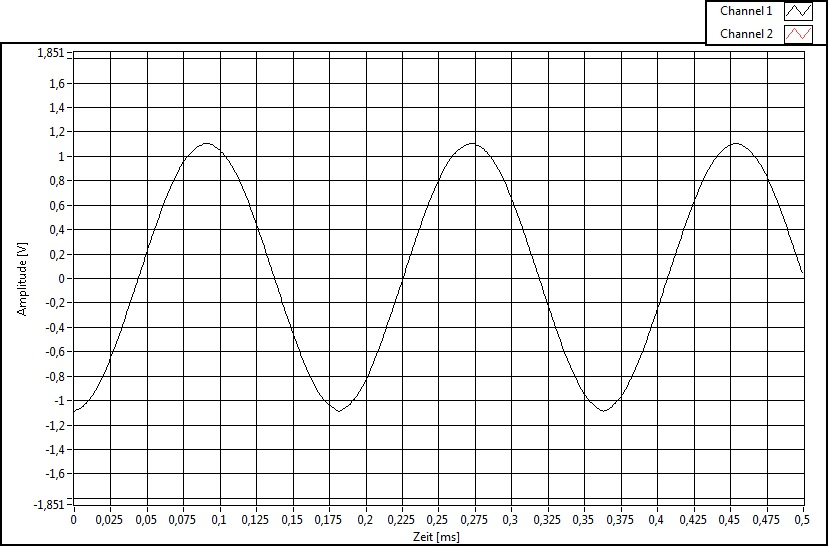
\includegraphics[width=\textwidth]{Aufgabe1Scope1.jpg}
  \caption{Darstellung des Signals am Eingang des Codec.}
  \label{fig:SinusFunktionsGen}
\end{figure}


Dieses Signal wurde, wie alle weiteren mit dem \textit{VI FFT \& FRF \& Scope} 
aufgezeichnet.\pagebreak

In der Vorbereitung wurde die Funktion copyData() erstellt, die sich wie folgt 
aufbaut:
\begin{adjustbox}{width=\textwidth,keepaspectratio}
\lstinputlisting[title=copydata.c]{copydata.c}
\end{adjustbox}

Wie man leicht sieht werden die Werte die der Codec liefert kopiert und in den iDMARxBuffer 
fortlaufend geschrieben, bis dieser voll ist. 
In dem Fall wird an der ersten Position des Buffer erneut angefangen und die alten Werte werden überschrieben.
Software VisualDSP++ biete die Möglichkeit den DSP zu debuggen.\pagebreak


Stoppt man nun den Durchlauf kann man, wie in der Aufgabenstellung beschrieben 
die aktuellen Werte des iDMARxBuffer ausleiten und mit MatLab visualisieren. 
\begin{figure}[!htb]
  \centerline{
    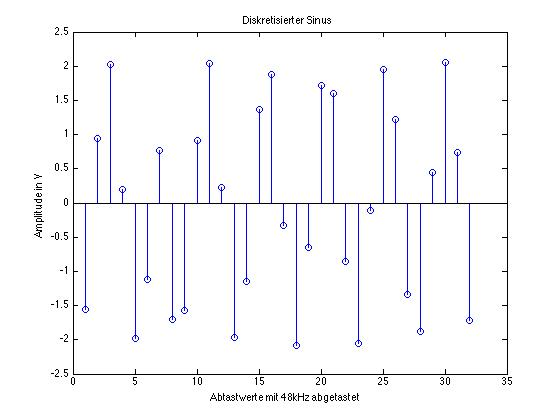
\includegraphics[width=\textwidth]{DiskreterSinusMatlab.jpg}}
      \caption{Darstellung der Datenreihe aus den Werten des DSP.}
      \label{fig:SinusMatlab}
\end{figure}

\section{Auswertung}
Aus Abbildung ~\ref{fig:SinusFunktionsGen} war ein Sinussignal zu erwarten, in Abbildung~\ref{fig:SinusMatlab} ist diese Sinussignal wieder zu erkennen.\\\par
Die Amplitude des Signals beträgt 1446560512 in der Registerdarstellung des DPS. Um diesen Wert exakt ermitteln zu können, wurde die Matlab-Funktion max() 
verwendet
Für die normierte Kreisfrequenz wird der Ansatz 
\begin{equation}\label{normierteKreisfrequenz}
 \omega_0=\frac{2\pi}N 
\end{equation}  

verwendet und führt bei 18 Messwerten in 2 Perioden (es folgt \begin{math}N=\frac{18}{2}\end{math}) zu 
\begin{equation*}
 \omega_0=\frac{2\pi}9 
\end{equation*}

Da die Diskreten Amplitudenwerte im 32-bit-Integer Format vorliegen, müssen sie in eine Spannung umgerechnet werden, hierzu sind die Daten des EVB erforderlich.
Der Codec hat eine Auflösung von 24-bit bei einer Spitze-Spitze-Spannung \begin{math}V_{ss}=6,16V\end{math}.\pagebreak
Es gilt zur Berechnung der Amplitudenspannung \begin{math}V_{Amp}\end{math}
\begin{equation}\label{umrechnungRegisterzuSpannung}
  V_{Amp}=\frac{V_{ADC}*V_{ss}}{2*2^{Registerbreite-1}}
\end{equation} 
Dies ergibt bei einem Registerwert von 1446560512 eine Spannung von 
\begin{math}V_{ss_{max}}=2,0579V\end{math}\\\par
Es ist an dieser Stelle nicht nachweisbar ob es sich bei dem gemessenen Maximalwert auch um das tatsächliche Maximum handelt, 
da der Abtastzeitpunkt nicht unbedingt der Zeitpunkt des lokalen Hochpunktes war.
Auch ist die Frequenz des Ursprungssignals nur näherungsweise zu ermitteln, da die Abtastfrequenz kein ganzzahliges vielfaches der Signalfrequenz ist. 
Um letztgenannten Fehler zu minimieren wurden in erster Annäherung die Abtastwerte über 4 Perioden ermittelt.
Die Frequenz des abgetasteten Sinus lässt sich mit
\begin{equation}\label{freqAbgetastetesSignal}
 f_0=\frac{f_s}N 
\end{equation}  
zu \begin{math}f_0 = 5,3kHz\end{math} berechnen, da der Codec mit 48kHz 
abtastet.\\\par
Aus der Messung ergibt sich grafisch eine Amplitude von \begin{math}V_{ss}=1,1V\end{math} und eine Frequenz von 5,5kHz. 
Die Abweichungen sind u.A. der Messung aus o.g. Gründen und des Ablesens geschuldet. 
Eine weitere Fehlerquelle bildet die interne Schaltung des EVB, so wie der Verstärker zwischen Eingang und ADC.
